\documentclass{standalone}
\usepackage[dvipsnames]{xcolor}
\usepackage{pgfplots}

\pgfplotsset{compat=1.9}
\usetikzlibrary{arrows.meta}
\usepgfplotslibrary{fillbetween}

\newif\ifgoalset
\goalsetfalse

\begin{document}
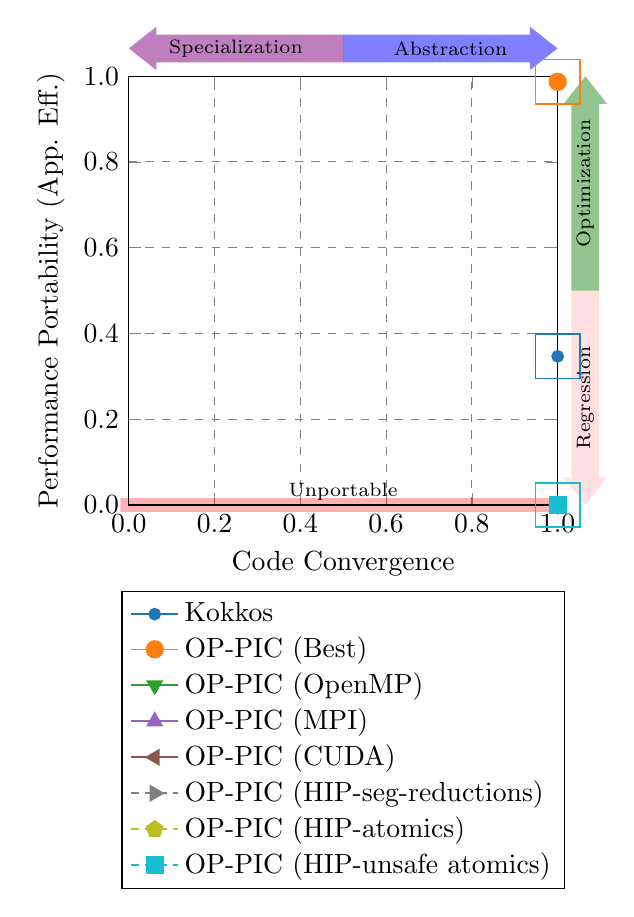
\begin{tikzpicture}
    % Set the size of the plot
    \newcommand{\plotheight}{200pt}
    \newcommand{\plotwidth}{200pt}

    % Application Efficiency or Architectural Efficiency?
    \newcommand{\plotylabel}{Performance Portability (App. Eff.)}

    % If a goal has been set, set the x and y values here
    \ifgoalset
        \newcommand{\goalx}{1.0}
        \newcommand{\goaly}{1.0}
    \fi

    %%% Define colors for applications
    \definecolor{Kokkos}{rgb}{0.12156862745098039, 0.4666666666666667, 0.7058823529411765}
    \definecolor{OPPICBest}{rgb}{1.0, 0.4980392156862745, 0.054901960784313725}
    \definecolor{OPPICOpenMP}{rgb}{0.17254901960784313, 0.6274509803921569, 0.17254901960784313}
    \definecolor{OPPICMPI}{rgb}{0.5803921568627451, 0.403921568627451, 0.7411764705882353}
    \definecolor{OPPICCUDA}{rgb}{0.5490196078431373, 0.33725490196078434, 0.29411764705882354}
    \definecolor{OPPICHIPsegreductions}{rgb}{0.4980392156862745, 0.4980392156862745, 0.4980392156862745}
    \definecolor{OPPICHIPatomics}{rgb}{0.7372549019607844, 0.7411764705882353, 0.13333333333333333}
    \definecolor{OPPICHIPunsafeatomics}{rgb}{0.09019607843137255, 0.7450980392156863, 0.8117647058823529}
    
    %%% Plot the space first, for the arrows to have reference points
    \begin{axis}
        [
            xticklabel style={/pgf/number format/.cd, fixed, fixed zerofill, precision=1},
            yticklabel style={/pgf/number format/.cd, fixed, fixed zerofill, precision=1},
            width=\plotwidth,
            height=\plotheight,
            name=NavChart,
            xlabel={Code Convergence},
            ylabel=\plotylabel,
            xmin=0,
            xmax=1,
            ymin=0,
            ymax=1,
            xmajorgrids=true,
            ymajorgrids=true,
            grid style={dashed,gray},
        ]
    \end{axis}

    %%% Plot the guide arrows around the plot

    % Specialization Arrow
    \begin{scope}[transparency group, opacity=0.5]
        \draw [violet, line width=1em, -{Triangle[width=1.5em,length=1em]}] ([yshift=1em]NavChart.north) -- ([yshift=1em]NavChart.north west) ;
    \end{scope}
    \draw [draw opacity=0.0] ([yshift=1em]NavChart.north) -- ([yshift=1em]NavChart.north west) node [midway, color=black, font=\scriptsize] {Specialization} ;

    % Abstraction Arrow
    \begin{scope}[transparency group, opacity=0.5]
        \draw [blue, line width=1em, -{Triangle[width=1.5em,length=1em]}] ([yshift=1em]NavChart.north) -- ([yshift=1em]NavChart.north east) ;
    \end{scope}
    \draw [draw opacity=0.0] ([yshift=1em]NavChart.north) -- ([yshift=1em]NavChart.north east) node [midway, color=black, font=\scriptsize] {Abstraction} ;

    % Regression Arrow
    \begin{scope}[transparency group, opacity=0.5]
        \draw [pink, line width=1em, -{Triangle[width=1.5em,length=1em]}] ([xshift=1em]NavChart.east) -- ([xshift=1em]NavChart.south east) ;
    \end{scope}
    \draw [draw opacity=0.0] ([xshift=1em]NavChart.east) -- ([xshift=1em]NavChart.south east) node [midway, rotate=90, color=black, font=\scriptsize] {Regression} ;

    % Optimization Arrow
    \begin{scope}[transparency group, opacity=0.5]
        \draw [ForestGreen, line width=1em, -{Triangle[width=1.5em,length=1em]}] ([xshift=1em]NavChart.east) -- ([xshift=1em]NavChart.north east) ;
    \end{scope}
    \draw [draw opacity=0.0] ([xshift=1em]NavChart.east) -- ([xshift=1em]NavChart.north east) node [midway, rotate=90, color=black, font=\scriptsize] {Optimization} ;

    % Unportable Line
    \begin{scope}[transparency group, opacity=0.3]
        \draw [red, line width=0.5em] ([xshift=-0.3em]NavChart.south west) -- ([xshift=0.3em]NavChart.south east) ;
    \end{scope}
    \draw [draw opacity=0.0] (NavChart.south west) -- (NavChart.south east) node [midway, color=black, yshift=0.5em, font=\scriptsize] {Unportable} ;

    % Plot each variant on the plot in a separate axis on top of the previous axis.
    \begin{axis}
        [
            xmin=0,
            xmax=1,
            ymin=0,
            ymax=1,
            ticks=none,
            width=\plotwidth,
            height=\plotheight,
            legend style={at={(0.5,-0.2)},anchor=north},
            legend cell align={left}
        ]

        \addplot+ [semithick, Kokkos, mark options={fill=Kokkos}, mark=*, mark options={style={solid}}] coordinates { (1.0, 0.34667564714504634) };
        \addlegendentry{Kokkos}
        \addplot+ [forget plot, semithick, Kokkos, only marks, mark size=8, mark=square] coordinates { (1.0, 0.34667564714504634) };

        \addplot+ [semithick, OPPICBest, mark options={fill=OPPICBest}, mark=*, mark options={style={solid}, scale=1.5}] coordinates { (1.0, 0.9867180475617445) };
        \addlegendentry{OP-PIC (Best)}
        \addplot+ [forget plot, semithick, OPPICBest, only marks, mark size=8, mark=square] coordinates { (1.0, 0.9867180475617445) };

        \addplot+ [semithick, OPPICOpenMP, mark options={fill=OPPICOpenMP}, mark=triangle*, mark options={style={solid}, scale=1.5, rotate=180}] coordinates { (1.0, 0.0) };
        \addlegendentry{OP-PIC (OpenMP)}
        \addplot+ [forget plot, semithick, OPPICOpenMP, only marks, mark size=8, mark=square] coordinates { (1.0, 0.0) };

        \addplot+ [semithick, OPPICMPI, mark options={fill=OPPICMPI}, mark=triangle*, mark options={style={solid}, scale=1.5}] coordinates { (1.0, 0.0) };
        \addlegendentry{OP-PIC (MPI)}
        \addplot+ [forget plot, semithick, OPPICMPI, only marks, mark size=8, mark=square] coordinates { (1.0, 0.0) };

        \addplot+ [semithick, OPPICCUDA, mark options={fill=OPPICCUDA}, mark=triangle*, mark options={style={solid}, scale=1.5, rotate=90}] coordinates { (1.0, 0.0) };
        \addlegendentry{OP-PIC (CUDA)}
        \addplot+ [forget plot, semithick, OPPICCUDA, only marks, mark size=8, mark=square] coordinates { (1.0, 0.0) };

        \addplot+ [semithick, OPPICHIPsegreductions, mark options={fill=OPPICHIPsegreductions}, mark=triangle*, mark options={style={solid}, scale=1.5, rotate=270}] coordinates { (1.0, 0.0) };
        \addlegendentry{OP-PIC (HIP-seg-reductions)}
        \addplot+ [forget plot, semithick, OPPICHIPsegreductions, only marks, mark size=8, mark=square] coordinates { (1.0, 0.0) };

        \addplot+ [semithick, OPPICHIPatomics, mark options={fill=OPPICHIPatomics}, mark=pentagon*, mark options={style={solid}, scale=1.5}] coordinates { (1.0, 0.0) };
        \addlegendentry{OP-PIC (HIP-atomics)}
        \addplot+ [forget plot, semithick, OPPICHIPatomics, only marks, mark size=8, mark=square] coordinates { (1.0, 0.0) };

        \addplot+ [semithick, OPPICHIPunsafeatomics, mark options={fill=OPPICHIPunsafeatomics}, mark=square*, mark options={style={solid}, scale=1.5}] coordinates { (1.0, 0.0) };
        \addlegendentry{OP-PIC (HIP-unsafe atomics)}
        \addplot+ [forget plot, semithick, OPPICHIPunsafeatomics, only marks, mark size=8, mark=square] coordinates { (1.0, 0.0) };

        
        % Plot a goal region if a goal has been set.
        \ifgoalset
            \path [name path=A] (axis cs:\goalx, \goaly) -- (axis cs:1.0, \goaly) ;
            \path [name path=B] (axis cs:\goalx, 1.0) -- (axis cs:1.0, 1.0) ;
            \addplot [yellow] fill between [ of=A and B ] ;
            \addplot+ [blue, thick, dashed, mark=none] coordinates { (0, \goaly) (1, \goaly) };
            \addplot+ [blue, thick, dashed, mark=none] coordinates { (\goalx, 0) (\goalx, 1) };
        \fi

    \end{axis}
\end{tikzpicture}
\end{document}